% =============================================================
%  PROCEDURE  (sections/03_procedure.tex)
% =============================================================

\chapter{Procedure}

% Describe WHAT YOU DID in enough detail that someone else could
% replicate the work. Use subsections to organise distinct phases
% or methods. Keep subsection names consistent with those you will
% use in the Results chapter.

% ----- Subsection 1 -------------------------------------------
\section{Part 1}
\label{sec:proc_part1}
\subsection{Well Design}
This subsecion describes the design of the default well. Because the wells were not drilled, it is necessary to specify the tubing and production casing.
Is was informed that the inflow can be modeled as a single-phase steady-state solution of the Darcy equation for a vertical fully penetrating well.
The Productivity Index (PI) equation is given by:
\begin{equation}
    PI = \frac{q_{liq}}{\bar{p} - p_{wf}} = \frac{kh}{141.2 B_o \mu_o \left[\ln{\left(\frac{r_e}{r_{wf}}\right)}-0.5 + S\right]} \quad \text{STB/d/psi}
\end{equation}
Where $q_{liq}$ is the liquid flow rate in STB/d, $\bar{p}$ is the average reservoir pressure, $p_{wf}$ is the bottom hole flowing pressure (psi), $k$ is the permeability in mD, $h$ is the thickness of the reservoir in ft, $B_o$ is the oil formation volume factor (RB/STB), $\mu_o$ is the oil viscosity (cP), $r_e$ is the drainage radius (ft), $r_{wf}$ is the wellbore radius (ft) and $S$ is the skin factor.
The reservoir properties are given in Table \ref{tab:reservoir_properties}.

% =============================================================
%  RESERVOIR & FLUID PROPERTIES TABLE
%  Drop this block into any section file, e.g. 03_procedure.tex
%  Requires: booktabs, siunitx (add to main.tex preamble)
% =============================================================

% Add to main.tex preamble if not already present:
% \usepackage{booktabs}
% \usepackage{siunitx}

\begin{table}[htbp]
    \centering
    \caption{Reservoir and Fluid Properties}
    \label{tab:reservoir_properties}
    \begin{tabular}{l l r l}
        \toprule
        \textbf{Parameter} & \textbf{Symbol} & \textbf{Value} & \textbf{Unit} \\
        \midrule
        \multicolumn{4}{l}{\textit{Reservoir Conditions}} \\
        \midrule
        Reservoir pressure       & $\bar{P}$  & 3800          & psia          \\
        Reservoir temperature    & $T$         & 200           & $^\circ$F     \\
        \midrule
        \multicolumn{4}{l}{\textit{Rock Properties}} \\
        \midrule
        Permeability             & $k$         & 40            & mDarcy        \\
        Net pay thickness        & $h$         & 150           & ft            \\
        Drainage radius          & $r_e$       & 372           & ft            \\
        Skin factor              & $S$         & 0             & --            \\
        \midrule
        \multicolumn{4}{l}{\textit{Fluid Properties}} \\
        \midrule
        API gravity              & API         & 45            & $^\circ$API   \\
        Oil viscosity (res.)     & $\mu_o$     & 0.902         & cp            \\
        Gas specific gravity     & $\gamma_g$  & 0.6636        & --            \\
        Gas-oil ratio            & GOR         & 800           & scf/STB       \\
        Bubble point pressure    & $P_b$       & 3800          & psia @ 200$^\circ$F \\
        Formation volume factor  & $B_o$       & 1.2           & RB/STB @ $P_b$ \\
        \midrule
        \multicolumn{4}{l}{\textit{Production Constraints}} \\
        Maximum rroduction rate & $q_{\max}$   & 45,000        & STB/d         \\
        Number of production wells          & $N_{wells}$   & 7             & --            \\
        Minimum wellhead pressure & $P_{wh,\min}$  & 1200          & psia          \\
        \bottomrule
    \end{tabular}
\end{table}

It was stated that the drilling and completion costs are highly sensitive to the wellbore radius ($r_{wf}$). So, first, we should
try to finde the minimum tubing size that allows to produce the maximum flow rate for each development scenario. The maximum flow rate per well 
was defined as $q_{\max} / N_{wells}$, which is 6428.57 STB/d. The Figure \ref{fig:pi_x_radii} shows the relationship between the Productivity Index and the wellbore radius for the given reservoir and fluid properties.
From the plot, it is observed that the PI range is between 5.5 and 6.0 STB/d/psi for a casing OD between 4.5 and 7.75 inches (9\% improvement) but the difference between the 7 and 7.75 inches is only 0.1 STB/d/psi (1.7\% improvement). 
\begin{figure}[htbp]
    \centering
    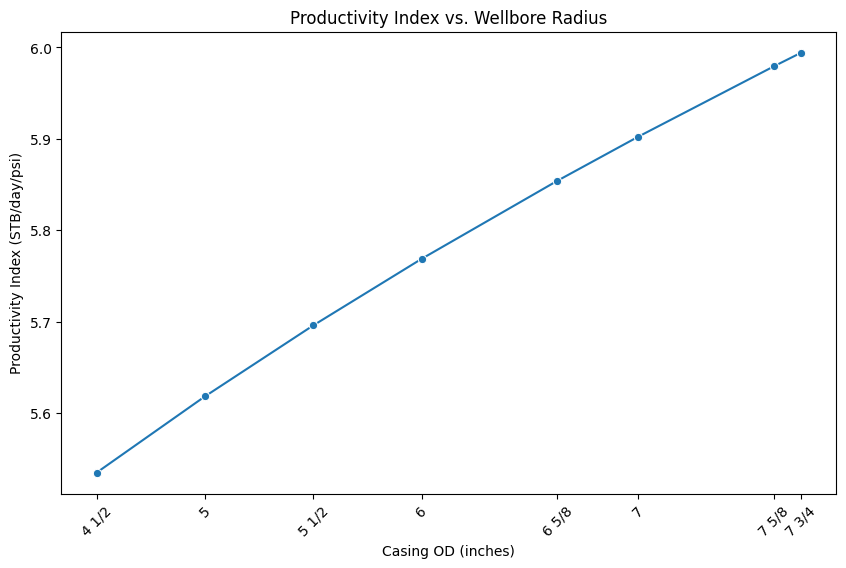
\includegraphics[width=0.7\textwidth]{figs/pi_vs_radius.png}
    \caption{Productivity Index vs. Wellbore Radius}
    \label{fig:pi_x_radii}
\end{figure}
It was also assumed that the tubing size should be $0.8 r_{wf}$. The behaviour of the Producivity Index is shown in Figure \ref{fig:pi_x_tubing_radius}. Because the PI is just a function of the wellbore radius, the plot is the same as in Figure \ref{fig:pi_x_radii}, but with a different x-axis. 
\begin{figure}[htbp]
    \centering
    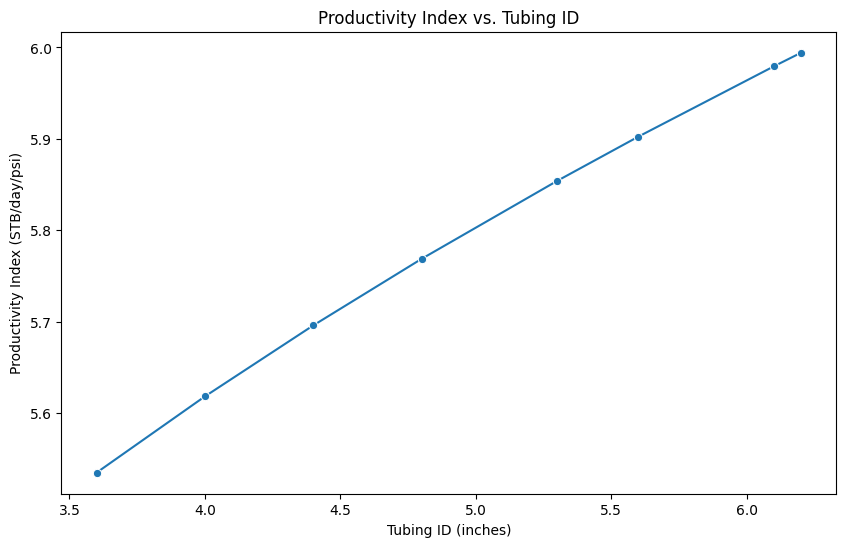
\includegraphics[width=0.7\textwidth]{figs/pi_vs_tubing_radius.png}
    \caption{Productivity Index vs. Tubing Radius}
    \label{fig:pi_x_tubing_radius}
\end{figure}

It was adivised that the asphaltene precipitation occurs at a pressure of 1100 psis, so the minimum wellhead pressure should be at least 1200 psia. 
A wellbore model of Well 1 was created using Pipesim and the impact of tubing ID was evaluated. The results are shown in Figure \ref{fig:well1_q_x_tubing_radius}. It can be observed that the flow rate is higher than the maximum allowed for all tubing sizes, but the 4.5 inches tubing has a flow rate of 7000 STB/d, which is much higher than the maximum allowed. The 7 inches tubing has a flow rate of 6500 STB/d, which is also higher than the maximum allowed but closer to it. The 7.75 inches tubing has a flow rate of 6400 STB/d, which is just below the maximum allowed. Therefore, the 7 inches tubing was selected for Well 1.
\begin{figure}[htbp]
    \centering
    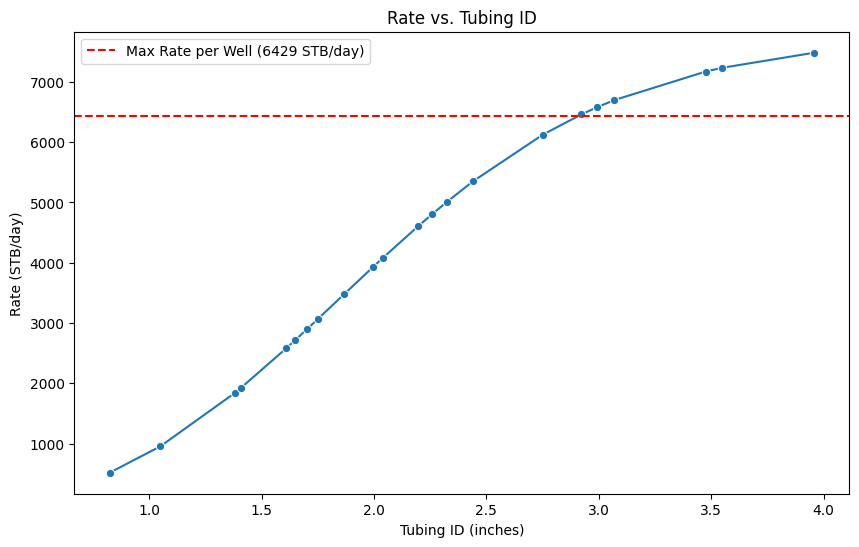
\includegraphics[width=0.7\textwidth]{figs/rate_vs_tubing_id.png}
    \caption{Flow Rate vs. Tubing Radius for Well 1}
    \label{fig:well1_q_x_tubing_radius}
\end{figure}
The minimum tubing ID that allows to produce the maximum flow rate was 2.922 inches, which corresponds to a tubing OD of 3.5 inches. Because it is necessary to have as least 1 inch of annular space between the tubing and the casing, the minimum casing ID should be 5.5 inches. 
A 5.5 ID casing corresponds to a 6.625 inches OD casing. In our project, we decided to use a 7 inches OD casing due to the best productivity index and the fact that it is a common casing size. A larger casing size would not be justified because the improvement in the productivity index is not significant and it would increase the drilling and completion costs.
The production forecast predicts the water cut will improve and it was necessary to evaluate the impact of water cut on the flow rate. The results are shown in Figure \ref{fig:well1_q_x_water_cut}. It can be observed that the well rate does not produce the maximum allowed flow rate for a water cut higher than 10\%. 
\begin{figure}[htbp]
    \centering
    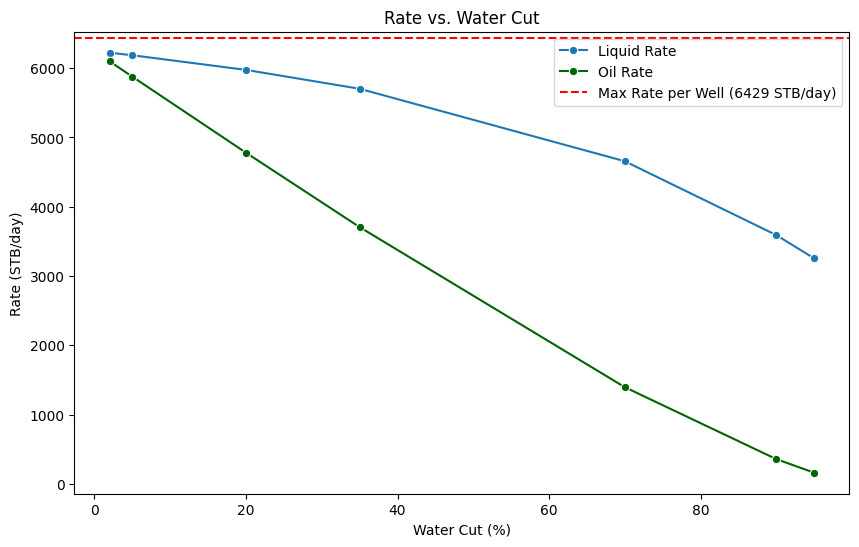
\includegraphics[width=0.7\textwidth]{figs/rate_vs_watercut.png}
    \caption{Flow Rate vs. Water Cut for Well 1}
    \label{fig:well1_q_x_water_cut}
\end{figure}
So, it was observed that when the well starts to produce water, the maximum liquid rate is not achieved, so it is necessary to implement artificial lift. 
The only artificial lift option available is the gas-lift. The gas-lift rate was evaluated for different water cuts and the results are shown in Figure \ref{fig:well1_gas_lift_rate_x_water_cut}. 
It is observed that the minimum gas-lift rate that allows to produce the maximum liquid rate for all water cuts is 1.5 MMscf/d. 
\begin{figure}[htbp]
    \centering
    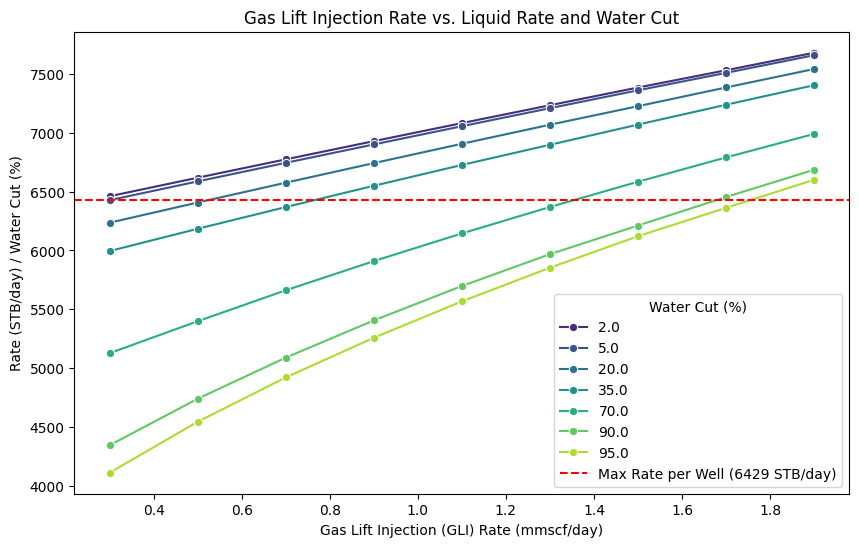
\includegraphics[width=0.7\textwidth]{figs/rate_vs_gas_lift.png}
    \caption{Gas-Lift Rate and Water Cut vs. Liquid Rate for Well 1}
    \label{fig:well1_gas_lift_rate_x_water_cut}
\end{figure}
% ----- Subsection 2 -------------------------------------------
\section{Part 2}
\label{sec:proc_phase2}
It was also analyzed the impact of the gas-lift rate and water cut on the wellhead temperature. The results are shown in Figure \ref{fig:well1_q_x_gas_lift_and_temp}. 
It was not informed the minimum wellhead temperature, but for this configuration, the wellhead temperature is above 176$^\circ$F for all water cuts and gas-lift rates.
\begin{figure}[htbp]
    \centering
    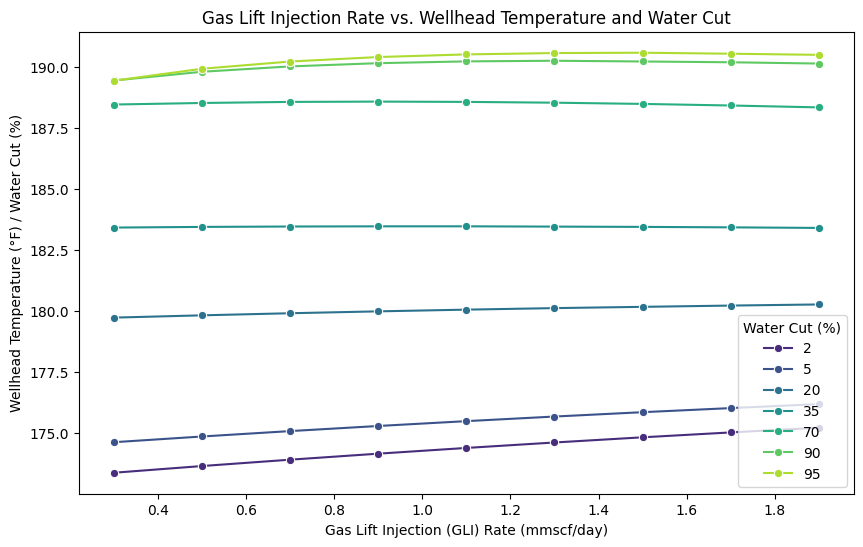
\includegraphics[width=0.7\textwidth]{figs/rate_vs_gas_lift_and_temp.png}
    \caption{Wellhead Temperature vs. Gas-Lift Rate and Water Cut for Well 1}
    \label{fig:well1_q_x_gas_lift_and_temp}
\end{figure}


\lipsum[6] % Replace with description of second method / phase

% Add or remove \section{} blocks as needed.
